\documentclass[10pt,twocolumn,letterpaper]{article}

\usepackage{iccv}
\usepackage{caption}
\usepackage{times, graphicx, amsmath, amssymb, subcaption}
\usepackage[]{algorithm2e}

% Include other packages here, before hyperref.

% If you comment hyperref and then uncomment it, you should delete
% egpaper.aux before re-running latex.  (Or just hit 'q' on the first latex
% run, let it finish, and you should be clear).
\usepackage[pagebackref=true,breaklinks=true,colorlinks,bookmarks=false]{hyperref}

%\iccvfinalcopy % *** Uncomment this line for the final submission

\def\iccvPaperID{1341} % *** Enter the ICCV Paper ID here
\def\httilde{\mbox{\tt\raisebox{-.5ex}{\symbol{126}}}}

% Pages are numbered in submission mode, and unnumbered in camera-ready
\ificcvfinal\pagestyle{empty}\fi
\begin{document}

%%%%%%%%% TITLE
\title{Mosaicing Scenes with Vacant Spaces (Supplementary Material)}

\maketitle

\textbf{Description}
We have added output in the supplementary material which we were not able
to include in the ``Experiments and Results'' section of original paper due to
the page restriction. Additionally, we have put video recordings (recorded
through quadcopter) in folder named ``video''. 

The file `teaser.avi' refers to results shown in Figure 1 in main paper.
The file `lady1.avi' refers to results shown in Figure 7 in main paper.
Finally, the file `greenRed.avi' refers to results shown in Figure 8 in main
paper.
 

\begin{figure*}[h!]
\centering
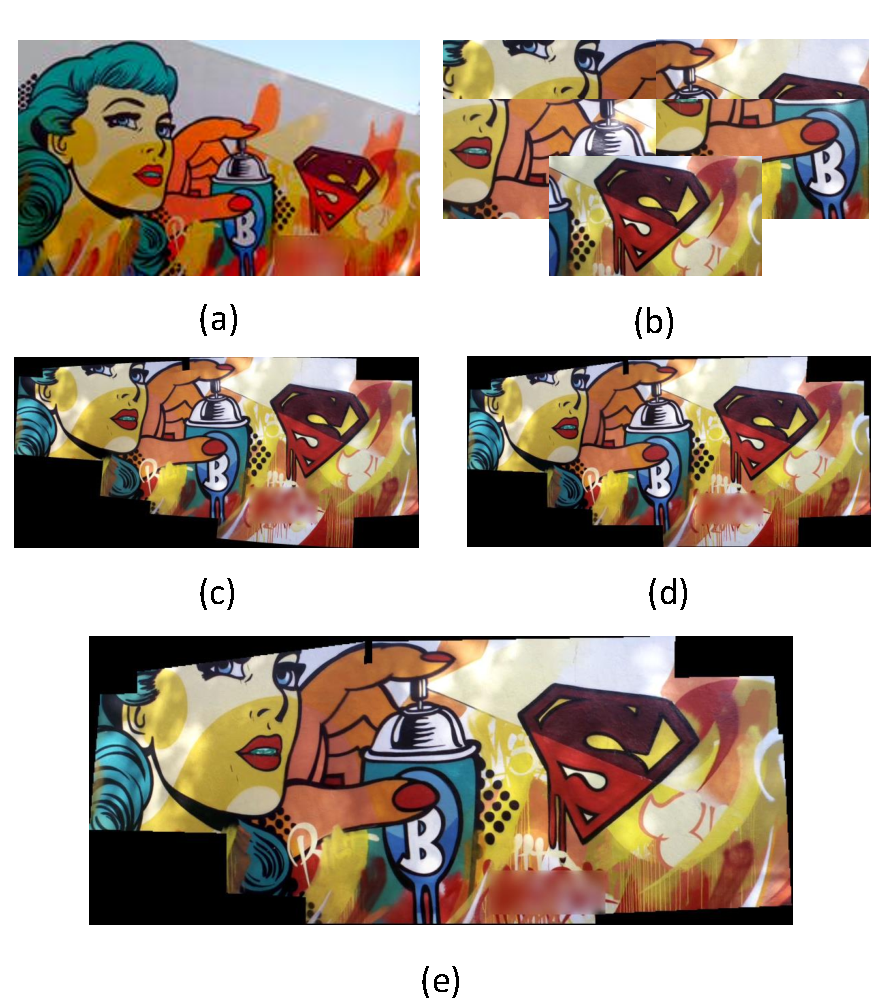
\includegraphics[width=0.87\linewidth]{figures/lady2.pdf}
\caption{ (a) Uniformly sampled images from an outdoor video
  expedition.  (b) Salient image selection from the set of
  approximately 9000 images using positional information. (c) Autostitch output
  (d) Adobe Photoshop CS6 output (e) Our output }
\label{fig:validResults}
\end{figure*}

The input stream (videos/lady2.avi) had about 9000 images. The selection
algorithm pruned the video into $N=15$ images. The scene as captured by a smartphone can also be seen in
Figure~\ref{fig:validResults}(a). A sample of the
selected images are seen in Figure~\ref{fig:validResults}(b).
Figure~\ref{fig:validResults}(c,d,e) shows the comparison of outputs of state
of the art stitchers with the output of our algorithm. As there are no vacant
spaces, our stitching algorithm's output is similar to that of Autostitch as
well as Photoshop.

\begin{figure*}[h!]
\centering
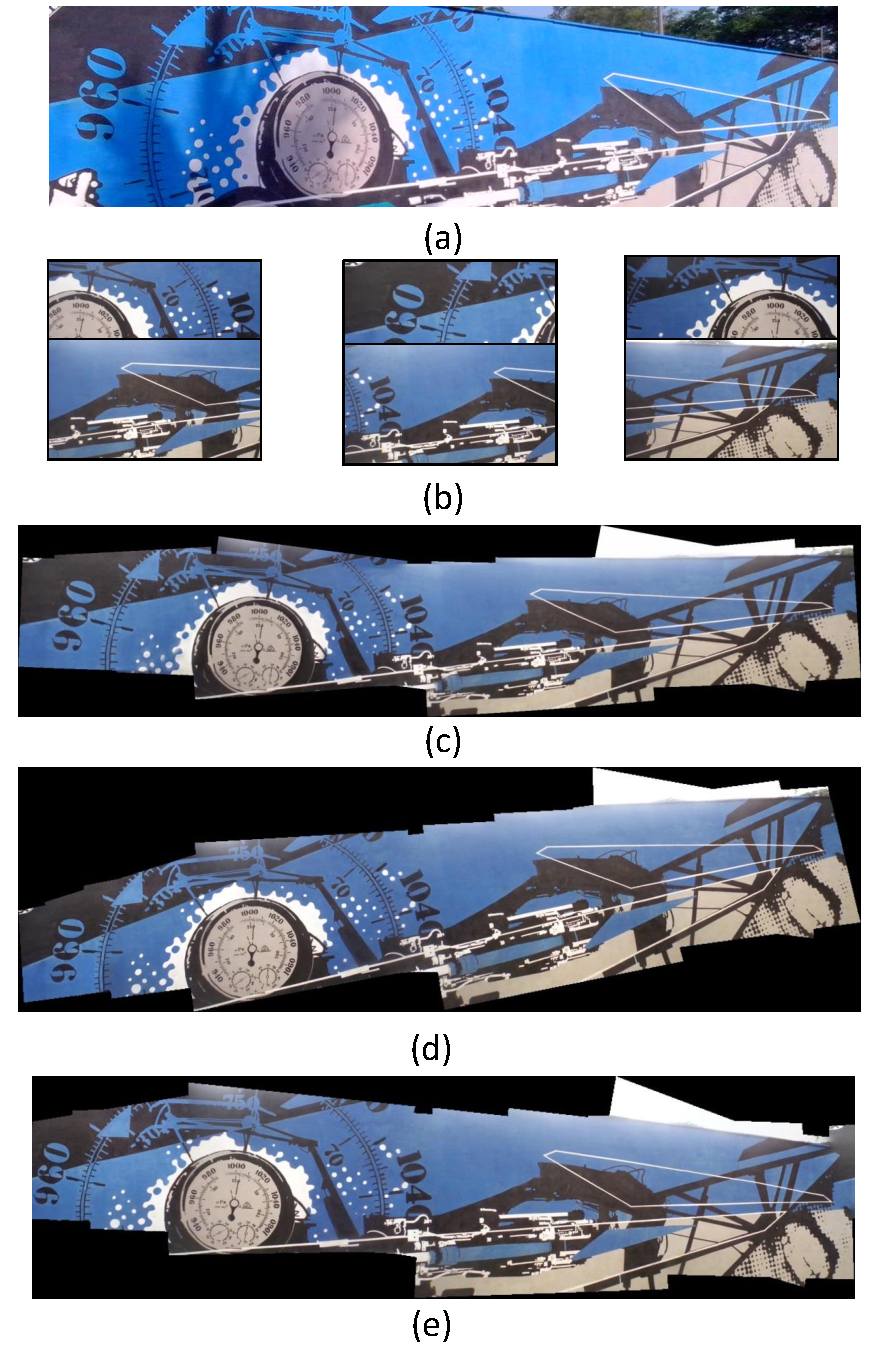
\includegraphics[width=0.8\linewidth]{figures/longwall.pdf}
\caption{ (a) Uniformly sampled images from an outdoor video
  expedition.  (b) Salient image selection from the set of
  approximately 9000 images using positional information. (c) Autostitch output
  (d) Adobe Photoshop CS6 output (e) Our output }
\label{fig:validResults1}
\end{figure*}

The input stream (videos/longwall.avi) had about 4000 images. The selection
algorithm pruned the video into $N=19$ images.
The scene as captured by a smartphone can also be seen in
Figure~\ref{fig:validResults1}(a). A sample of the
selected images are seen in Figure~\ref{fig:validResults1}(b).
Figure~\ref{fig:validResults1}(c,d,e) shows the comparison of outputs of state
of the art stitchers with the output of our algorithm. As there are no vacant
spaces, our stitching algorithm's output is similar to that of Autostitch as
well as Photoshop.

\begin{figure*}[h!]
\centering
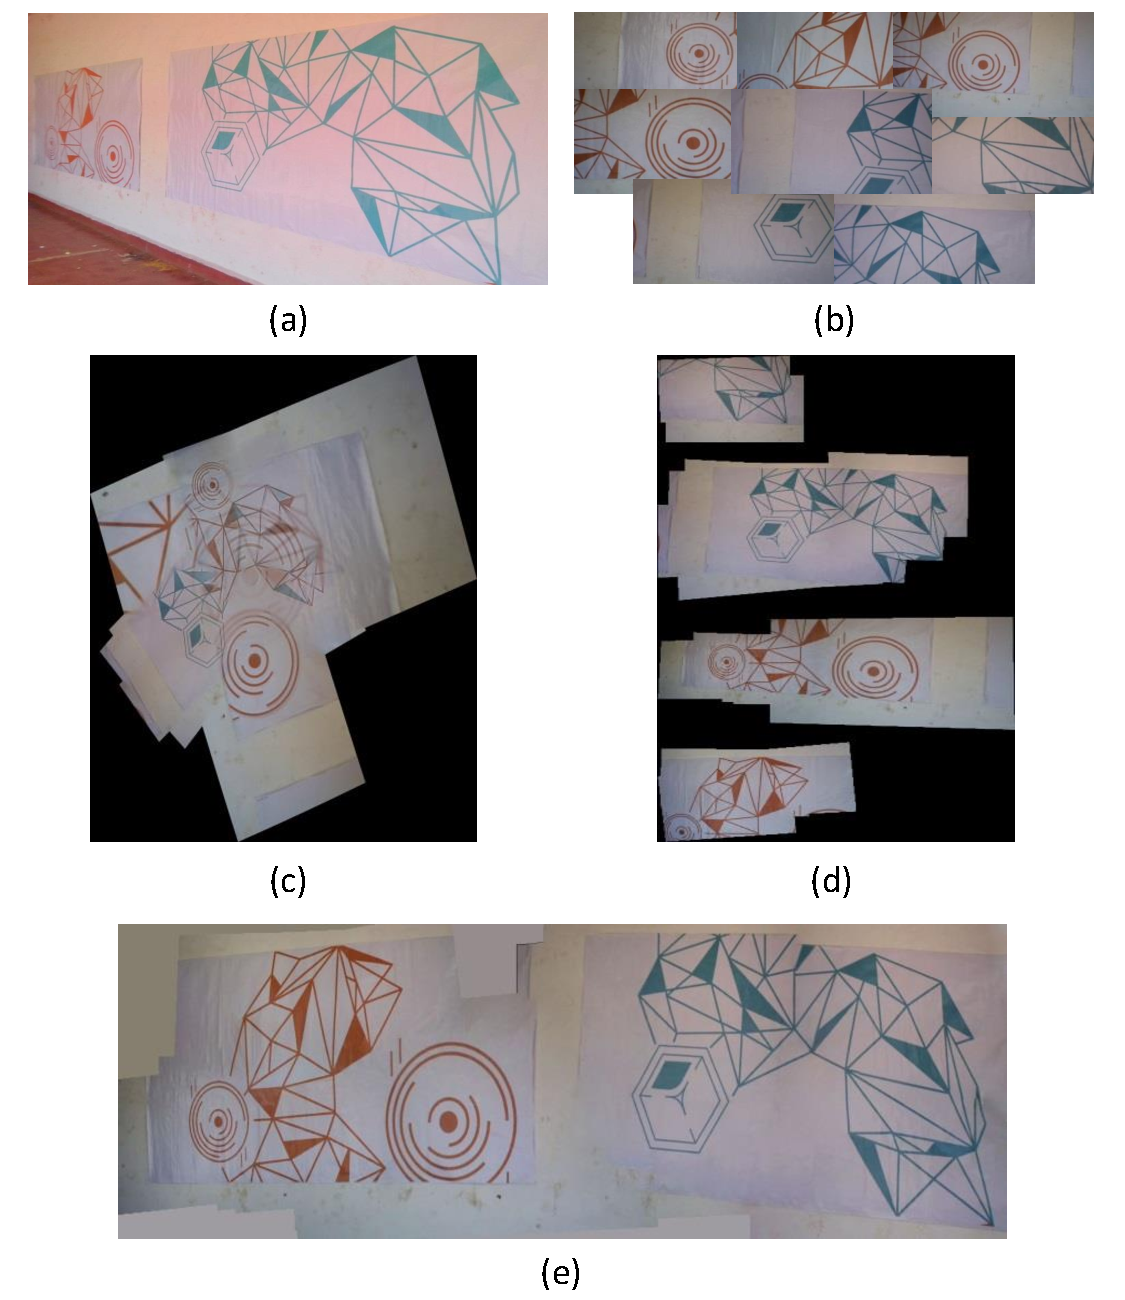
\includegraphics[width=0.85\linewidth]{figures/orange_blue.pdf}
\caption{(a) An outdoor scene captured by a standard camera in an
  exhibition. The approach to the area is normally cordoned off and one
  needs permission to get a quadcopter to take the picture.  Notice a
  significant gap between the two posters.  (b) Pruned images from the
  quadcopter video using our saliency algorithm. (c) Output of
  Autostitch on the selected images. The mosaic is not reasonable
  presumably because of the confusion in features. (d) Output of Adobe
  Photoshop CS6 on the selected images. The vacant space posed a
  problem to the feature matching algorithm, so instead of a mosaic,
  individual pieces were output as mini-panoramas (e) Our output on
  the selected images. We are able to join two posters (separated by
  vacant space) using IMU data.}
\label{fig:results1}
\end{figure*}

The input stream (videos/orangeBlue.avi) had about 9100 images. The selection
algorithm pruned the video into $N=28$ images. The scene as captured by a smartphone can also be seen in
Figure~\ref{fig:results1}(a). A sample of the
selected images are seen in Figure~\ref{fig:results1}(b).
Figure~\ref{fig:results1}(c,d,e) shows the comparison of outputs of state
of the art stitchers with the output of our algorithm. As there are vacant
spaces, Autostitch as well as Photoshop are not able to stitch images
accurately. But, as we are using IMU data, our output is closest to input scene. 

\begin{figure*}[h!]
\centering
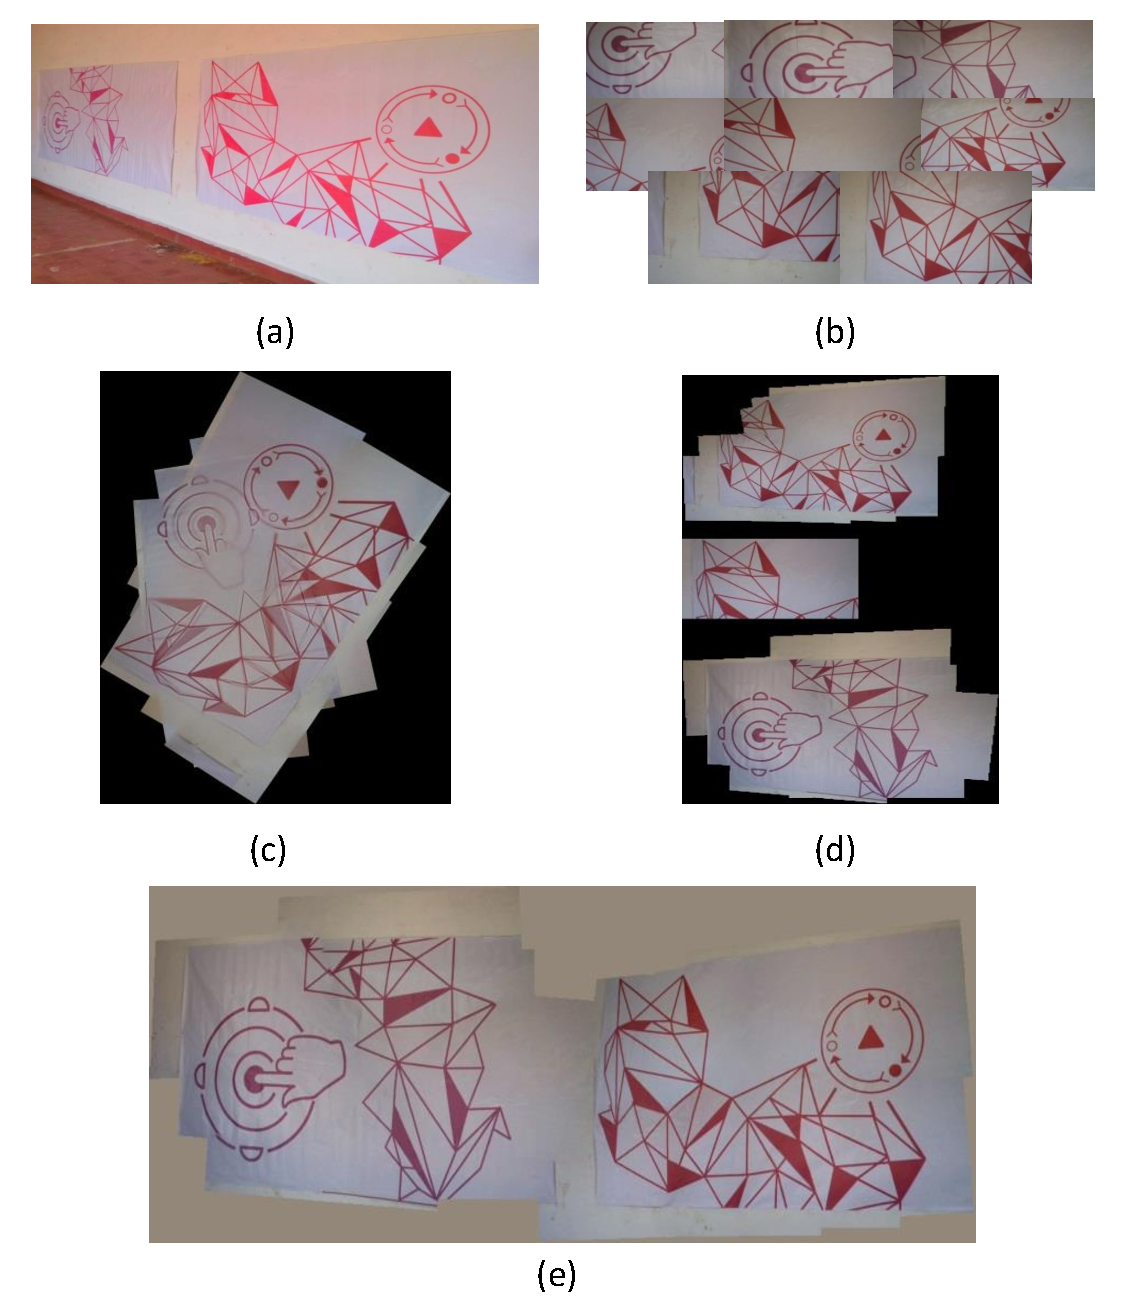
\includegraphics[width=0.85\linewidth]{figures/Purple_red.pdf}
\caption{(a) An outdoor scene captured by a standard camera in an
  exhibition. Notice a   significant gap between the two posters.  (b) Pruned
  images from the quadcopter video using our saliency algorithm. (c) Output of
  Autostitch on the selected images. The mosaic is not reasonable
  presumably because of the confusion in features. (d) Output of Adobe
  Photoshop CS6 on the selected images. The vacant space posed a
  problem to the feature matching algorithm, so instead of a mosaic,
  individual pieces were output as mini-panoramas (e) Our output on
  the selected images. We are able to join two posters (separated by
  vacant space) using IMU data.}
\label{fig:results2}
\end{figure*}
	
The input stream (videos/purpleRed.avi) had about 8500 images. The selection
algorithm pruned the video into $N=17$ images.The scene as captured by a smartphone can also be seen in
Figure~\ref{fig:results2}(a). A sample of the
selected images are seen in Figure~\ref{fig:results2}(b).
Figure~\ref{fig:results2}(c,d,e) shows the comparison of outputs of state
of the art stitchers with the output of our algorithm. As there are vacant
spaces, Autostitch as well as Photoshop are not able to stitch images
accurately. But, as we are using IMU data, our output is closest to input scene.
	
\end{document}